        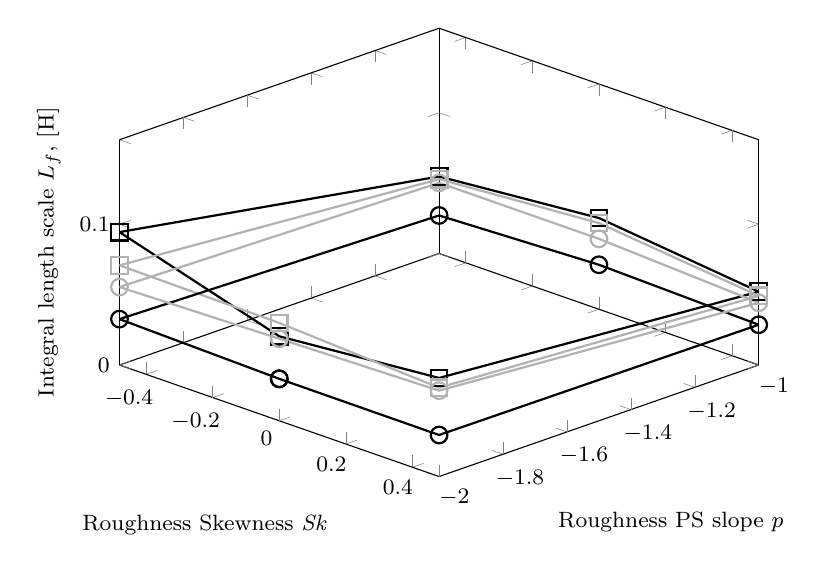
\begin{tikzpicture}[]
        \centering
        \begin{axis}[
        view={45}{35},
            ylabel={Roughness PS slope $p$},
            xlabel={Roughness Skewness \textit{Sk}},
			zlabel={Integral length scale $L_f$, [H]},
			%ztick={5.5,6,6.5,7,7.5},
			zmin=0,zmax=0.16,
            %ymin=0, ymax=0.16,
            width=.8\textwidth,
            height=.6\textwidth,
            label style={font=\footnotesize},
            tick label style={font=\footnotesize}
            ]
            
            
            
                                    \addplot3 [
            black,mark=square,thick, mark size=3pt
            ]
            coordinates{
            (0,-2,0.060)			
			(0.48,-2,0.0700)
			(0.48,-1,0.0521)
			(0,-1,0.0648)
			(-0.48,-1,0.0547)
			(-0.48,-2,0.0944)
            (0,-2,0.060)
			};
			\addplot3 [
            gray!60,mark=square,thick, mark size=3pt
            ]
            coordinates{
            (0,-2,0.0695)
			(0.48,-2,0.0631)
			(0.48,-1,0.0491)
			(0,-1,0.0612)
			(-0.48,-1,0.0528)
			(-0.48,-2,0.0708)
			(0,-2,0.0695)
            };
            
            
            
                                                \addplot3 [
            black,mark=o,thick, mark size=3pt
            ]
            coordinates{
            (0,-2,0.0298)		
			(0.48,-2,0.0295)
			(0.48,-1,0.0286)
			(0,-1,0.0316)
			(-0.48,-1,0.0270)
			(-0.48,-2,0.0326)
            (0,-2,0.0298)
			};
			\addplot3 [
            gray!60,mark=o,thick, mark size=3pt
            ]
            coordinates{
            (0,-2,0.0583)
			(0.48,-2,0.0610)
			(0.48,-1,0.0442)
			(0,-1,0.0500)
			(-0.48,-1,0.0502)
			(-0.48,-2,0.0554)
			(0,-2,0.0583)
            };
            
            
            
        \end{axis}
        \end{tikzpicture}